\chapter{Экспериментальная часть}

В данном разделе описаны замерные эксперименты и представлены результаты исследования.

\section{Технические характеристики}
Технические характеристики устройства, на котором выполнялся эксперимент \cite{bib:yandex}:
\begin{itemize}
	\item 96 ГБ оперативной памяти;
	\item процессор Intel Ice Lake (96 ядер);
    \item операционная система Ubuntu 20.04.
\end{itemize}

\section{Постановка исследования}
Целью исследования является определение зависимости времени генерации изображения лесистой местности от количества потоков, выделенных на выполнение данной задачи. Исследование проводилось для количества потоков, не превышающих 400, так как уже на этом значении скорость работы алгоритма не увеличивается с увеличением числа потоков. Во время проведения исследования устройство было подключено к блоку питания, и не нагружено программами, кроме операционной системы и средств разработки. 

\section{Средства исследования}
Время синтеза изображения измеряется с использованием библиотеки \texttt{chrono} \cite{bib:chrono}. Измеряется реальное время, что особо важно с учетом того, проводится исследования параллельных вычислений.

\section{Результаты исследования}
Полученные результаты измерения описаны в таблице \ref{table:speed}. Нулевое количество потоков означает отсутствие создания дополнительных потоков.
\newpage

\begin{table}[h!]
  \caption{\label{table:speed} Результаты замеров времени (в мс)}
  \begin{center}
    \begin{tabular}{|r|r|}
      \hline
      Количество потоков & Время\\ \hline
		0 & 28288 \\ \hline
		1 & 28817 \\ \hline
		2 & 24448 \\ \hline
		5 & 11734 \\ \hline
		10 & 6135 \\ \hline
		20 & 3214 \\ \hline
		30 & 2185 \\ \hline
		40 & 1741 \\ \hline
		60 & 1349 \\ \hline
		80 & 1100 \\ \hline
		100 & 1058 \\ \hline
		120 & 1004 \\ \hline
		140 & 1048 \\ \hline
		160 & 981 \\ \hline
		190 & 925 \\ \hline
		230 & 899 \\ \hline
		260 & 869 \\ \hline
		290 & 848 \\ \hline
		320 & 889 \\ \hline
		350 & 877 \\ \hline
		400 & 872 \\ \hline
    \end{tabular}
  \end{center}
\end{table}

\newpage

На рис. \ref{img:plot} приведен график, показывающий зависимость времени выполнения программы от количества выделенных потоков.

\begin{figure}[h!]
	\centering
    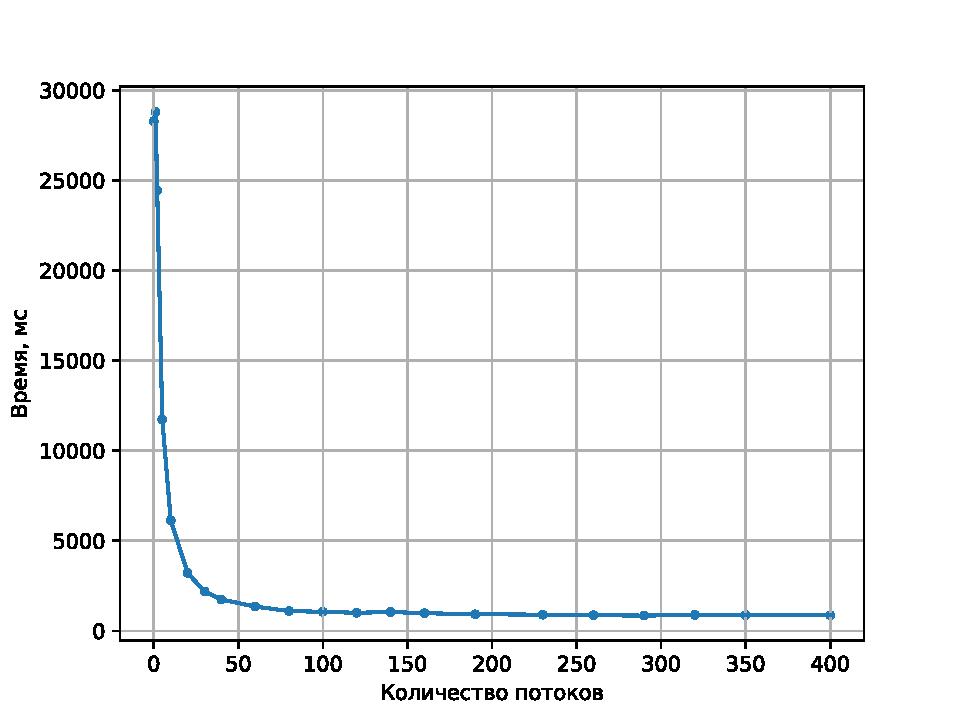
\includegraphics[width=0.95\linewidth]{plot.pdf}
    \caption{График зависимости времени выполнения от количество потоков}
    \label{img:plot}
\end{figure}

\newpage